\externaldocument{../4/chapter_modeling}
\label{chapter:appendix}
\startchapter{Communication Identification Algorithms}
\label{chapter:alo}
In the Modeling Chapter, I elaborate the definition of the communications and the strategy of the communication identification. There are several major steps in the identification strategy. In this chapter, I list developed the algorithms for the key steps in the identification strategy.  

\section{Communication Identification Process}
In the first section of this chapter, I define what is a communication. The identification of the communications from a dual-trace should be able to identify the concerned communications as well as all the components defined in it. The section section in this chapter investigate the characteristics of the communication methods which is the key factor affecting the verification of the transferred data of a communication. From the trace analysis point of view, channel open events are essential to identify an endpoint while all other events are optional in the identification.

The identification contains seven major steps:
\begin{itemize}
 \item Locate all events
 \item Identify the endpoints from the channel open events
 \item Group the related events into streams, send streams and receive streams, then bind them to the corresponding endpoint
 \item Match the endpoints to the communications
 \item For reliable communication, verify if the send data union in the stream of one endpoint match the receive data union in the stream of the other endpoint; For unreliable communication, try to match the send and receive events of both endpoints 
 \item Construct and organize all the retrieved data of the communication 
 \item Present the identified communications to the user
\end{itemize}

\section{Communication Methods' Implementation in Windows}\label{windows}
Finally I discuss the implementation of the communication methods and draw the function lists of the event types of some concerned communication methods. The function list of a communication method is one of the inputs for the communication identification.

In this section, the implementations of the four communication methods in Windows system are investigated. The goal of this investigation is to determine the system functions for the events in the communication definition and summarize the necessary parameters of all the communication events to further identify a communication. Each function call will be considered as an event. The channel opening mechanism is essential for identifying the endpoints and further the communication. Hence the channel opening mechanisms of each method are described in detail and represented in diagrams. 

I reviewed the Windows APIs of the communication methods and their example code. For each communication method, a system function list is provided for reference. These lists contain function names, essential parameters. These functions are supported in most Windows operating systems, such as Windows 8, Window 7. 

Windows API set is very sophisticated and multiple solutions are provided to fulfil a communication method. It is impossible to enumerate all solutions for each communication method. I only give the most basic usage provided in Windows documentation. Therefore, the provided system function lists for the events should not be considered as the only combination or solution for each communication method. With the understanding of the model, it should be fairly easy to draw out lists for other solutions or other communication methods. 

Moreover, the instances of this model only demonstrate Windows C++ APIs. This model may be generalizable to other operating systems with the effort of understanding the APIs of those operating systems.

\subsection{Windows Calling Convention}
The Windows calling convention is important to know in this research. The communication identification relies not only on the system function names but also the key parameter values. In the assembly level execution traces, the parameter values is captured in the memory changes of the instructions. The memory changes are recognized by the register names or the memory address. The calling convention helps us to understand where the parameters are stored so that we can find them in the memory change map in the trace.

Calling Convention is different for operating systems and the programming language. Based on the need of this work, we only list the Microsoft* x64 calling convention for interfacing with C/C++ style functions:\par
\begin{enumerate}  
\item RCX, RDX, R8, R9 are used for integer and pointer arguments in that order left to right.
\item XMM0, 1, 2, and 3 are used for floating point arguments.
\item Additional arguments are pushed on the stack left to right. \ldots 
\item Parameters less than 64 bits long are not zero extended; the high bits contain garbage.
\item Integer return values (similar to x86) are returned in RAX if 64 bits or less.
\item Floating point return values are returned in XMM0.
\item Larger return values (structs) have space allocated on the stack by the caller, and RCX then contains a pointer to the return space when the callee is called. Register usage for integer parameters is then pushed one to the right. RAX returns this address to the caller.
\end{enumerate}

\subsection{Named Pipes}
In Windows, a named pipe is a communication method for the pipe server and one or more pipe clients. The pipe has a name, can be one-way or duplex. Both the server and clients can read or write into the pipe.\cite{WinNamedpipe} In this work, I only consider one server versus one client communication. One server to multiple clients scenario can always be divided into multiple server and client communications thanks to the characteristic that each client and server communication has a separate conduit. The server and client are endpoints in the communication. We call the server ``server endpoint" while the client ``client endpoint".  The server endpoint and client endpoint of a named pipe share the same pipe name, but each endpoint has its own buffers and handles. 

There are two modes for data transfer in the named pipe communication method, synchronous and asynchronous.  Modes affect the functions used to complete the send and receive operation. I list the related functions for both synchronous mode and asynchronous mode. The create channel functions for both modes are the same but with different input parameter value. The functions for send and receive message are also the same for both cases. However, the operation of the send and receive functions are different for different modes. In addition, an extra function \textit{GetOverlappedResult} is being called to check if the sending or receiving operation finish, the output message will be stored in the overlap structure whose memory address saved in the function's output parameter Overlap Structure Address. Table\ref{synfunctions} lists the functions of the events for synchronous mode while Table\ref{asynfunctions} lists the functions of the events for the asynchronous mode for a Named pipe communication.

    \begin{table}[H]
        \centering
        \caption{Function List  of events for Synchronous Named Pipe}
        \label{synfunctions}
        \begin{tabular}{|l|l|l|l|l|}
            \hline
             \multirow{2}{*}{\textbf{Event}} &
               \multicolumn{2}{c|}{\textbf{Server Endpoint}} &
               \multicolumn{2}{c|}{\textbf{Client Endpoint}} \\
             \cline{2-5}
              & \textbf{Function}& \textbf{Parameters} & \textbf{Function} & \textbf{Parameters}  \\
             \hline
             \multirow{2}{*}{{\textbf{Channel Open}}}
             &\multirow{2}{*}{{CreateNamedPipe}} &  RAX: File Handler & \multirow{2}{*}{CreateFile} &  RAX: File Handler\\
              \cline{3-3} \cline{5-5}
             &&  RCX: File Name &  &  RCX: File Name\\
            \hline
             \multirow{3}{*}{{\textbf{Send}}}
             &\multirow{3}{*}{WriteFile} &  RCX: File Handle & \multirow{3}{*}{WriteFile} &  RCX: File Handle\\
              \cline{3-3} \cline{5-5}
             &&  RDX: Buffer Address &  &  RDX: Buffer Address\\
                           \cline{3-3} \cline{5-5}
             & &  R9: Message Length &  &  R9: Message Length\\
            \hline
             \multirow{3}{*}{{\textbf{Receive}}}
             & \multirow{3}{*}{ReadFile}&  RCX: File Handle & \multirow{3}{*}{ReadFile} &  RCX: File Handle\\
              \cline{3-3} \cline{5-5}
              &&  RDX: Buffer Address &  &  RDX: Buffer Address\\
                           \cline{3-3} \cline{5-5}
             & &  R9: Message Length &  &  R9: Message Length\\
            \hline
           {{\textbf{Channel Close}}}
             &{CloseHandle} & {RCX: File Handler} & {CloseHandle} & {RCX: File Handler}\\
            \hline
        \end{tabular}
    \end{table}

    \begin{table}[H]
        \centering
        \caption{Function List  of events for Asynchronous Named Pipe}
        \label{asynfunctions}
        \begin{tabular}{|l|l|l|l|l|}
            \hline
             \multirow{2}{*}{\textbf{Event}} &
               \multicolumn{2}{c|}{\textbf{Server Endpoint}} &
               \multicolumn{2}{c|}{\textbf{Client Endpoint}} \\
             \cline{2-5}
              & \textbf{Function}& \textbf{Parameters} & \textbf{Function} & \textbf{Parameters}  \\
             \hline
             \multirow{2}{*}{{\textbf{Channel Open}}}
             &\multirow{2}{*}{{CreateNamedPipe}} &  RAX: File Handler & \multirow{2}{*}{CreateFile} &  RAX: File Handle\\
              \cline{3-3} \cline{5-5}
             &&  RCX: File Name &  &  RCX: File Name\\
            \hline
             \multirow{3}{*}{{\textbf{Send}}}
             &\multirow{3}{*}{WriteFile} &  RCX: File Handle & \multirow{3}{*}{WriteFile} &  RCX: File Handle\\
              \cline{3-3} \cline{5-5}
             &&  RDX: Buffer Address &  &  RDX: Buffer Address\\
                           \cline{3-3} \cline{5-5}
             & &  R9: Message Length &  &  R9: Message Length\\
            \hline
            \multirow{3}{*}{{\textbf{Receive}}}
             & \multirow{3}{*}{ReadFile}&  RAX: File Handle & \multirow{3}{*}{ReadFile} &  RCX: File Handle\\
              \cline{3-3} \cline{5-5}
              &&  RDX: Buffer Address &  &  RDX: Buffer Address\\
                           \cline{3-3} \cline{5-5}
             & &  R9: Message Length &  &  R9: Message Length\\
              \hline
               \multirow{2}{*}{{\textbf{Receive}}}
             & \multirow{2}{*}{GetOverlapped-}&  RCX: File Handler & \multirow{2}{*}{GetOverlapped-} &  RCX: File Handler\\
              \cline{3-3} \cline{5-5}
             &  \multirow{2}{*}{Result} &  RDX:  Overlap  &  \multirow{2}{*}{Result }&  RDX:  Overlap \\
              &  &  Structure address &  &  Structure Address\\
            \hline                       
            \textbf{Channel Close}
             &{CloseHandle} &{RCX: File Handler} & {CloseHandle} &  {RCX: File Handler}\\
            \hline
        \end{tabular}
    \end{table}
    
A named pipe server is responsible for the creation of the pipe, while clients can connect to the pipe after it was created. The creation and connection of a named pipe returns the handle ID of that pipe. These handler Ids will be used later when data is being sent or received to a specified pipe. Figure\ref{namedpipeopen} shows the channel set up process for a Named Pipe communication.
\begin{figure}[H]
\centerline{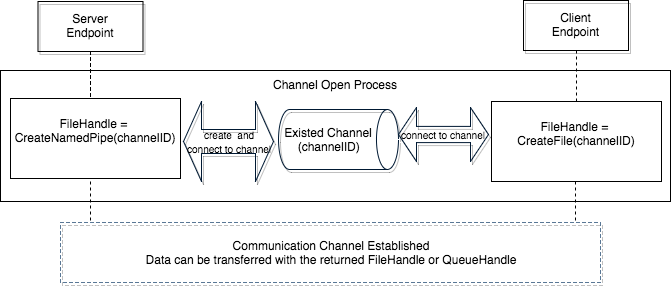
\includegraphics[scale=0.55]{Figures/namepipechannelopen}}
 \caption{Channel Open Process for a Named Pipe}
\label{namedpipeopen}
\end{figure}

\subsection{Message Queue}
Similar to Named Pipe, Message Queue's implementation in Windows also has two modes, synchronous and asynchronous. Moreover, the asynchronous mode further divides into two operations, one with callback function while the other without. With the callback function, the callback function would be called when the send or receive operations finish. Without callback function, the general function \textit{MQGetOverlappedResult} should be called by the endpoints to check if the message sending or receiving operation finish, the output message will be stored in the overlap structure whose memory address saved in the function's output parameter Overlap Structure Address. Table\ref{msmqsynfunctions} lists the functions for synchronous mode while Table\ref{msmqasynfunctionscallback} and Table\ref{msmqasynfunctions} list the functions for the asynchronous mode with and without callback. 

    \begin{table}[H]
        \centering
        \caption{Function List  of events for Synchronous MSMQ}
        \label{msmqsynfunctions}
        \begin{tabular}{|l|l|l|}
            \hline
             \textbf{Event} & \textbf{Function}& \textbf{Parameters}  \\
             \hline
             \multirow{2}{*}{{\textbf{Channel Open}}}
             &\multirow{2}{*}{{MQOpenQueue}} &  RAX: Queue Handler\\
              \cline{3-3} 
             & &  RCX: Queue Format Name\\
            \hline
             \multirow{2}{*}{{\textbf{Send}}}
             &\multirow{2}{*}{MQSendMessage} &  RCX: Queue Handle \\
              \cline{3-3} 
             &&  RDX: Message description structure Address \\
            \hline
             \multirow{2}{*}{{\textbf{Receive}}}
             & \multirow{2}{*}{MQReceiveMessage}&  RCX: Queue Handle \\
              \cline{3-3} 
              &&  R9: Message description structure Address \\
            \hline
            \textbf{Channel Close} &MQCloseQueue & RCX: Queue Handler \\
            \hline
        \end{tabular}
    \end{table}


    \begin{table}[H]
        \centering
        \caption{Function List of events for Asynchronous MSMQ with Callback}
        \label{msmqasynfunctionscallback}
        \begin{tabular}{|l|l|l|}
            \hline
             \textbf{Event} & \textbf{Function}& \textbf{Parameters}  \\
             \hline
             \multirow{2}{*}{{\textbf{Channel Open}}}
             &\multirow{2}{*}{{MQOpenQueue}} &  RAX: Queue Handler\\
              \cline{3-3} 
             & &  RCX: Queue Format Name\\
            \hline
             \multirow{2}{*}{\textbf{Send}}
             &\multirow{2}{*}{MQSendMessage} &  RCX: Queue Handle \\
              \cline{3-3} 
             &&  RDX: Message description structure Address \\
            \hline
             \multirow{2}{*}{\textbf{Receive}}
             & \multirow{2}{*}{MQReceiveMessage}&  RCX: Queue Handle \\
              \cline{3-3} 
              &&  R9: Message description structure Address \\
             \hline
             \textbf{Receive}
              &CallbackFuncName&  Parameters for the callback function. \\
            \hline
            \textbf{Channel Close} &MQCloseQueue & RCX: Queue Handler \\
            \hline
        \end{tabular}
    \end{table}

    \begin{table}[H]
        \centering
        \caption{Function List  of events for Asynchronous MSMQ without Callback}
        \label{msmqasynfunctions}
        \begin{tabular}{|l|l|l|}
            \hline
             \textbf{Event} & \textbf{Function}& \textbf{Parameters}  \\
             \hline
             \multirow{2}{*}{{\textbf{Channel Open}}}
             &\multirow{2}{*}{{MQOpenQueue}} &  RAX: Queue Handler\\
              \cline{3-3} 
             & &  RCX: Queue Format Name\\
            \hline
             \multirow{2}{*}{{\textbf{Send}}}
             &\multirow{2}{*}{MQSendMessage} &  RCX: Queue Handle \\
              \cline{3-3} 
             &&  RDX: Message description structure Address \\
            \hline
             \multirow{2}{*}{{\textbf{Receive}}}
             & \multirow{2}{*}{MQReceiveMessage}&  RCX: Queue Handle \\
              \cline{3-3} 
              &&  R9: Message description structure Address \\
              \hline
              \textbf{Receive} 
              & MQGetOverlappedResult &  RCX: Overlap Structure address  \\
            \hline
            \textbf{Channel Close} &MQCloseQueue & RCX: Queue Handler \\
            \hline
        \end{tabular}
    \end{table}
    
The endpoints of the communication can create the queue or use the existing one. However, both of them have to open the queue before they access it. The handle ID returned by the open queue function will be used later on when messages are being sent or received to identify the queue. Figure\ref{msmqopen} shows the channel set up process for a Message Queue communication.
\begin{figure}[H]
\centerline{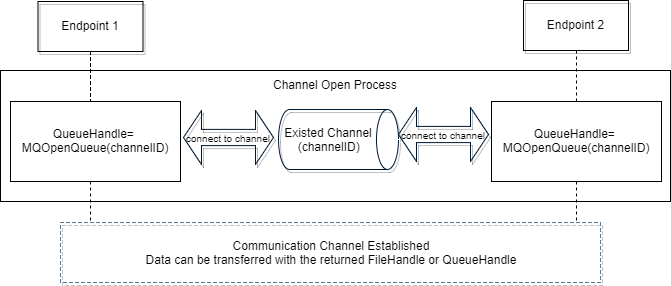
\includegraphics[scale=0.55]{Figures/msmqchannelopen}}
 \caption{Channel Open Process for a Message Queue}
\label{msmqopen}
\end{figure}
    
\subsection{TCP and UDP}
In Windows programming, these two methods shared the same set of APIs regardless the input parameter values and operation behaviour are different. In Windows socket solution, one of the two endpoints is the server while the other one is the client. Table \ref{tcpupdfunctions} lists the functions of a UDP or TCP communication. 
  \begin{table}[H]
        \centering
        \caption{Function List  of events for TCP and UDP}
        \label{tcpupdfunctions}
        \begin{tabular}{|l|l|l|l|l|}
            \hline
             \multirow{2}{*}{\textbf{Event}} &
               \multicolumn{2}{c|}{\textbf{Server Endpoint}} &
               \multicolumn{2}{c|}{\textbf{Client Endpoint}} \\
             \cline{2-5}
              & \textbf{Function}& \textbf{Parameters} & \textbf{Function} & \textbf{Parameters}  \\
             \hline
             \textbf{Channel Open}
             &socket&  RAX: Socket Handle & socket &  RAX: Socket Handle\\
             \hline
                \multirow{2}{*}{{\textbf{Channel Open}}}
              &\multirow{2}{*}{{bind}} &  RCX: Socket Handle & \multirow{2}{*}{connect} &  RCX: Socket Handle\\
              \cline{3-3} \cline{5-5}
             &&  RDX: Server Address $\&$ Port &  &  RDX: Server Address $\&$ Port\\
            \hline
                \multirow{3}{*}{{\textbf{Channel Open}}}
             &\multirow{3}{*}{{accept}} &  RAX: New Socket Handle && \\
              \cline{3-3} 
             &&  RCX:  Socket Handle &  & \\
             \cline{3-3} 
             &&  RDX: Client Address $\&$ Port &  &  \\
            \hline
             \multirow{2}{*}{{\textbf{Send}}}
             &\multirow{2}{*}{send} &  RCX: New Socket Handle & \multirow{2}{*}{send} &  RCX: Socket Handle\\
              \cline{3-3} \cline{5-5}
             &&  RDX: Buffer Address &  &  RDX: Buffer Address\\
           \hline
              \multirow{2}{*}{{\textbf{Receive}}}
             & \multirow{2}{*}{recv}&  RCX: New Socket Handle & \multirow{2}{*}{recv} &  RCX: Socket Handle\\
              \cline{3-3} \cline{5-5}
              &&  RDX: Buffer Address &  &  RDX: Buffer Address\\
            \hline
          {{\textbf{Channel Close}}}&
            {closesocket} & {RCX: New Socket Handle} &{closesocket} & {RCX: Socket Handle}\\
            \hline
        \end{tabular}
    \end{table} 
    
The communication channel is set up by both of the endpoints. The function \textit{socket} should be called to create their own socket on both endpoints. After the sockets are created, the server endpoint binds the socket to its service address and port by calling the function \textit{bind}. Then the server endpoint calls the function  \textit{accept} to accept the client connection. The client will call the function \textit{connect} to connect to the server. When the function \textit{accept} return successfully, a new socket handle will be generated and returned for further data transfer between the server endpoint and  the connected client endpoint. After all these operations are performed successfully, the channel is established and the data transfer can start. During the channel open stage, server endpoint has two socket handles, the first one is used to listen to the connection from the client, while the second one is created for real data transfer. Figure\ref{channelopen2} shows the channel open process for TCP and UDP.
    
\begin{figure}[H]
\centerline{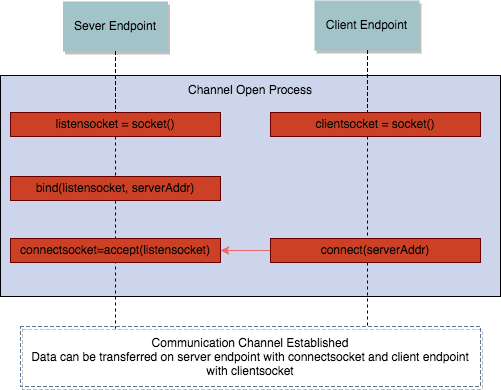
\includegraphics[scale=0.55]{Figures/tcpudpchannelopen}}
 \caption{Channel Open Model for TCP and UDP}
\label{channelopen2}    
\end{figure}


\section{Communication Event Locating in Assembly Execution Traces}
The goal of this research is to identify the communications from the dual-trace and present them to the user. The identification of all events of the communications from the execution trace would be the first step. Last section concludes communication events including system function names, parameters and the function calls relationship. This section will 1) discuss the basis of the execution traces. and 2) conclude how to retrieve the event information from the execution traces.

\subsection{Assembly Execution Trace}
The dual-trace being analysed are in assembly level. One dual-trace contains two execution traces. There is no timing information of these two traces which means we don't know the timestamps of the events of these two traces and can not match the events from both sides by time sequence. However the captured instructions in the trace are ordered in execution sequence. The execution traces contain all executed instructions as well as the corresponding changed memory by each instruction. Additionally, system calls are also captured by instruction id, which means if .dll or .exe files are provided, the system function calls can be identified with function names. Memory states can be reconstructed from the recorded memory changes to get the data information of the communication. 

\subsection{Event Information Retrieval}
For simplification, each function call is treated as an event. A function call in the trace starts from the function call instruction to the function return instruction. The input parameters' value and input buffer content should be retrieved from the memory state of the the function call instruction line while the return value, output parameters' value and output buffer content should be retrieved from the memory state of the function return instruction line. Tables in section \ref{windows} indicate all the functions of the communication methods as well as the concerned parameters. Following the windows calling convention, the concerned parameter value or buffer address can be found in the corresponding register or stack positions. The buffer content can be found in the memory address in the reconstructed memory state. 

\section{Event Locating Algorithm}
The concerned events in a communication are channel open, channel close, send and receive events. These events are identified as system function calls in this work. Each event can be completed by different function calls. For example, for the client endpoint in TCP communication method, both  \textit{socket} and \textit{connect} function call are considered to be the channel open events. The functions list for a communication method is needed as a input of this algorithm. Tables in Section\ref{windows} give the examples of function list of the events for some communication methods. The algorithm presented in this section is designed for locating all function calls provided in the function list as events of one communications method. If more than one communication methods are being investigated, this algorithm should be run multiple times, each for a method. Events in the output event list is sorted by time of occurrence. Since the function list usually contain a very small number of functions compared to the instruction line number in the execution trace, the time complexity of this algorithm is O(N+M) , N and M are the instruction line numbers of the two traces in the duel-trace.

\begin{algorithm}[H]
\DontPrintSemicolon
\caption{{\bf Event Locating Algorithm} \label{eventLocAlg}}
\KwIn{dual-trace, function list}
\KwOut{two event lists for two separative traces in the dual-trace}
$eventLists \leftarrow Map \langle String, List \langle Event\rangle \rangle$;\; 
\For{$trace \in dual$-$trace$}{
   $eventList \leftarrow List \langle Event\rangle$;\; 
   \While{not at end of trace}{
       \For{$f \in functionList$}{
           \If{Is function call of f}{ 
               find function return instruction line;\;          
               $event.inputs \leftarrow$ get input parameters from this instruction line;\;              
               $event.outputs \leftarrow$ get output parameters and return value from the return instruction line;\;
               $event.type \leftarrow f.eventType$;\;
               $eventList.add\left( event \right)$;\;
           }       
        }
    }
    $eventLists.add\left( eventList \right)$;\;
}
\KwRet $eventLists$;\;
\end{algorithm} 

\section{Endpoint Identification Algorithm}
The events located in the two traces may correspond to different endpoints, the next step in the strategy is to group them for each endpoints and furthermore group them into streams of the endpoints. The input of this algorithm is one of the event list for one trace from the Event Locating Algorithm. So this algorithm should be run separately for both traces in the dual-trace. Since the input event list is sorted by time of occurrence and the channel open events should always happen before other events, it is reasonable to assume the new endpoint can be identified by its first channel open function call. The identification for TCP and UDP server endpoints are slightly complicated than the other ones, due to its own channel open mechanism. The output of this algorithm is the endpoint list. Each endpoint in this list contains the stream which consist of the sub streams. The concepts of the stream and sub streams are defined in Section\ref{term}. 

\begin{algorithm}[H]
\DontPrintSemicolon
\caption{{\bf Endpoint Indentification Algorithm} \label{endpointIdentAlg}}
\KwIn{event list of a trace}
\KwOut{endpoint list}
$endpoints \leftarrow Map \langle String, List \langle EndPoint\rangle \rangle$;\; 
\For{$event \in eventList$}{
   \If{$event$ is a channel open event}{
      $handle \leftarrow$ get the handle identifier from the function parameter list;\;
      $endpoint \leftarrow endpoints.get\left( handle \right)$;\;
      \If{$event$ is an $accept\left( event \right)$ function call for TCP or UDP}{
         $newHandle \leftarrow$ get the second socket handle identifier which is the return value from the function parameter list;\;
         $endpoints.remove\left( handle \right)$;\;
         $endpoints.add\left( newHandle, endpoint \right)$;\;
      }
      
      \If{$endpoint$ is null}{
         $endpoint = New \enspace EndPoint\left( \right)$;\;
         $endpoints.add\left( hanele, endpoint \right)$;\;
      }
      $endpoint.openStream.add\left( event \right)$;\;
   }
   \If{$event$ is a channel send event}{
      $handle \leftarrow$ get the handle from the function parameter list;\;
      $endpoint \leftarrow endpoints.get\left( handle \right)$;\;
      \If{$endpoint$ is not $null$ and $endpoint.complete$ is $False$}{
         $endpoint.sendStream.add\left( event \right)$;\;
      }
   }
   \If{$event$ is a channel receive event}{
      $handle \leftarrow$ get the handle from the function parameter list;\;
      $endpoint \leftarrow endpoints.get\left( handle \right)$;\;
      \If{$endpoint$ is not $null$ and $endpoint.complete$ is $False$}{
         $endpoint.receiveStream.add\left( event \right)$;\;
      }
   }
   \If{$event$ is a channel close event}{
      $handle \leftarrow$ get the handle from the function parameter list;\;
      $endpoint \leftarrow endpoints.get\left( handle \right)$;\;
      \If{$endpoint$ is not null}{
         $endpoint.closeStream.add\left( event \right)$;\;
         $endpoint \leftarrow True$;\;
      }
   }         
}
\KwRet $endpoints$;\;
\end{algorithm} 

\section{Communication Identification Algorithm}
The communication identification algorithm aims at identifying all the communication of a concerned communication method from the dual-trace. The input of this algorithm is the two endpoint lists for both traces in the dual-trace from the `Endpoint Identification Algorithm'. The output of this algorithm is the communication list. Each communication recognized from the dual-trace contains two endpoints. The channel of a communication defined in Section\ref{definition} is not explicitly represented in the output but it was implicitly used in this algorithm. 

In the communication identification algorithm, it first try to match two endpoints to a channel only by their identifiers. In this level, the matching depends on channel open mechanisms which are different from communication method to communication method. For TCP and UDP the matching can be considered as local address and port of server endpoint matching with remote address and port of client endpoint. For Named Pipe, it uses the file name, while for Message Queue, it uses the queue name as the identifier for matching of two endpoints. 

The first level matching can not guarantee the exact endpoints matching and channel identification. There are two situations which false positive error might emerge. Take Named Pipe for example, the first situation is multiple(more than two) interacting programs shared the same file or queue as their own channel. Even though the channels are distinct for each communication, but the file or queue used is the same one. For example, the Named Pipe server is connected by two clients using the same file. In the server trace, there are two endpoints found. In each client trace, there is one endpoint found. In the channel identification algorithm for the dual-trace of server and client1, there will be two possible identified channels, one is the real used one for server and client1 communication while the other is the false positive error actually is for server and client2. The endpoint in client1's trace will be matched by two endpoints in the server's trace. The second situation is the same channel is reused by the different endpoints in the same programs. For example, the Named Pipe server and client finished the first communication and then closed the channel. After a while they re-open the same file again for another communication. Since the first level matching is only base on the identifiers and the first and the second communications have the same identifier since they used the same file. Similar situations can also happen in Message Queue, TCP and UDP communication methods. 

To reduce the false positive error, the second level matching should be applied, which is also being named as transmitted data verification algorithm. On top of the endpoint identifiers matching, further data verification should be applied to make sure the matching is reliable. This verification crossly compare the sent and received data of both endpoints in the first leve matching. If the transmitted data of the endpoints is considered to be identical, the matching is confirm, otherwise it was a false positive error. However, we still can not exclude all the false positive errors, due to the data transmitted in two communication can be identical. Figure\ref{secondlevelmatching} indicates the ineffective second level matching scenario and the effective one.

\begin{figure}[H]
\centerline{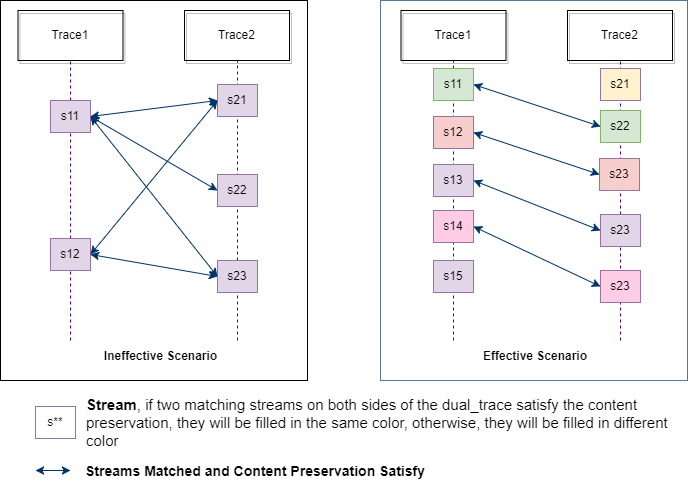
\includegraphics[scale=0.55]{Figures/secondlevelmatching}}
 \caption{Second Level Matching Scenarios}
\label{secondlevelmatching}
\end{figure}


The following subsections discuss the algorithms for these two level matching. In Section\ref{windows}, I elaborate the channel open process and the data transfer categories for the concerned communication methods. Based on the different channel process, two algorithms are developed for the communication identification, one is for Named Pipe and Message Queue, the other is for TCP and UDP. The inputs of the these two algorithms are the same, the two endpoint lists of the two traces of the analysing dual-trace. The output is the identified communications. Each communication contains the matched two endpoints from both sides of the traces and each endpoint contains its stream.

The data transfer characteristics divided the communication methods into reliable and unreliable transmissions. Named Pipe and TCP fall in the reliable category while Message Queue and UDP fall in the unreliable one. The second level matching algorithms are different for these two categories. The corresponding second level data matching algorithms are being used in the communication identification algorithms. The input of the transmitted data verification algorithms is the streams of both endpoint while the output a boolean to indicate if the transmitted data of this two endpoint streams are matched and the verified data.

\subsection{Communication Identification Algorithm for Named Pipe and Message Queue}
For Named Pipe and Message Queue, only one channel open function is being called for each endpoint. So in the below algorithm, when it try to get the channel open event from the $endpoint.openStream$ list, only one event should be found and return. The channel identifier parameters can be found in the $event.inputs$ of the channel open event. The identifier for Named Pipe is the file name of the pipe while for Message Queue is the format queue name of the queue. 

This algorithm finds out all the possible communications regardless some of them might be false positive errors. The called data verification algorithm is either ``Matching by Data Streams Algorithm" for Named Pipe or ``Matching by Data Events Algorithm" for Message Queue.

\begin{algorithm}[H]
\DontPrintSemicolon
\caption{{\bf Communication Indentification Algorithm for Named Pipe and Message Queue} \label{channelAlg1}}
\KwIn{two endpoint lists of the dual-trace}
\KwOut{communication list}
$communications \leftarrow Map \langle String, List \langle Communication \rangle \rangle$;\; 
\For{$endpoint1 \in endpointList1$}{
   $openEvent1 \leftarrow$ get the event from $endpoint1.openStream$, which should only contain one event;\;
   $channelId1 \leftarrow$ get the channel identifier from $openEvent1.inputs$;\;
   \For{$endpoint2 \in endpointList2$}{
      $openEvent2 \leftarrow$ get the event from $endpoint2.openStream$, which should only contain one event;\;
      $channelId2 \leftarrow$ get the channel identifier from $openEvent2.inputs$;\;
     \If{$channelId1 == channelId2$}{
         $DataVerified  \leftarrow $ Call the corresponding data verification algorithm.
         \If{$DataVerified == True$}{
            $communication = New \enspace Communication()$;\;
            $communication.endpoint1 = endpoint1$;\;
            $communication.endpoint2 = endpoint2$;\;
            $communication.dataMatch\leftarrow$ The output from data verification algorithm;\;
            $communications.add\left( communication \right)$;\;
         }    
      }
   }
}
\KwRet $channels$;\;
\end{algorithm} 


\subsection{Communication Identification Algorithm for TCP and UDP}
For TCP and UDP multiple functions are collaborating to create the final communication channel. The local address and port of the server endpoint and the remote address and port of the client endpoint are used to identify the channel. This algorithm first try to retrieve the local address and port of the server endpoint and remote address and port from client endpoint. Then it try to match two endpoints by comparing the local and remote address and port.

\begin{algorithm}[H]
\DontPrintSemicolon
\caption{{\bf Communication Indentification Algorithm for TCP and UDP} \label{channelAlg2}}
\KwIn{two endpoint lists of the dual-trace}
\KwOut{channel list}
$communications \leftarrow Map \langle String, List \langle Communication \rangle \rangle$;\; 
\For{$endpoint1 \in endpointList1$}{
   $bindEvent1 \leftarrow$ get the $bind\left( \right)$ function call related event from $endpoint1.openStream$;\;
   $connectEvent1 \leftarrow$ get the $connect\left( \right)$ function call related event from $endpoint1.openStream$;\;
   \For{$endpoint2 \in endpointList2$}{
      $bindEvent2 \leftarrow$ get the $bind\left( \right)$ function call related event from $endpoint2.openStream$;\;
      $connectEvent2 \leftarrow$ get the $connect\left( \right)$  function call related event from $endpoint2.openStream$;\;
    \If{$socketEvent1 !=null$ AND $socketEvent2 != null$}{
       \If{$bindEvent1 != null$ AND $connectEvent2 == null$}{
           $localServerAddr \leftarrow$ get the serverAddr parameter value from $bindEvent1.inputs$;\;
       }
       \ElseIf{$bindEvent2 == null$ AND $connectEvent1 != null$}{
           $remoteServerAddr \leftarrow$ get the serverAddr parameter value from $connectEvent1.inputs$;\; 
       }
       \Else{
          Break the inner For loop;\;
       }
       \If{$localServerAddr == remoteServerAddr$}{
          $DataVerified  \leftarrow $ Call the corresponding data verification algorithm.
          $communication = New \enspace Communication()$;\;
          $communication.endpoint1 = endpoint1$;\;
          $communication.endpoint2 = endpoint2$;\;
          $communication.dataMatch\leftarrow$ The output from data verification algorithm;\;
          $communications.add\left( communication \right)$;\;
       }
    }
   }
}
\KwRet $channels$;\;
\end{algorithm}

\subsection{Transmitted Data Verification for Named Pipe and TCP by Data Union}
As describe in Section\ref{reliable}, the data being received by one endpoint should always equal to or at least is sub string of the data being sent from the other endpoint in a communication for the reliable transmission methods, such as Named Pipe and TCP. So the transmitted data verification algorithm is in data union level. The send data union is retrieved by the conjunction of the input buffer content of the send events in the send stream of an endpoint. The receive data union is retrieved by the conjunction of the output buffer content of the receive events in the receive stream of the other endpoint. The input of this algorithm is the two endpoints from two traces which are being matched in the first level.
\begin{algorithm}[H]
\DontPrintSemicolon
\caption{{\bf Transmitted Verification by Data Union} \label{dataAlg1}}
\KwIn{two endpoints from each trace of the dual-trace}
\KwOut{send data union and receive data union of two endpoints}
\KwRet{Indicator of if transmitted data union are considered to be identical}
$send1 \leftarrow$ empty string;\;
$send2 \leftarrow$ empty string;\;
$recv1 \leftarrow$ empty string;\;
$recv2 \leftarrow$ empty string;\;
\For{$sendEvent \in endpoint1.sendStream$}{
   $sendmessage \leftarrow$ get the input buffer content from the $sendEvent.inputs$;\;
   $send1.append\left( sendmessage \right)$;\;
}
\For{$sendEvent \in endpoint2.sendStream$}{
   $sendmessage \leftarrow$ get the input buffer content from the $sendEvent.inputs$;\;
   $send2.append\left( sendmessage \right)$;\;
}
\For{$recvEvent \in endpoint1.receiveStream$}{
   $recvmessage \leftarrow$ get the output buffer content from the $recvEvent.outputs$;\;
   $recv1.append\left( sendmessage \right)$;\;
}
\For{$recvEvent \in endpoint2.receiveStream$}{
   $recvmessage \leftarrow$ get the output buffer content from the $recvEvent.outputs$;\;
   $recv2.append\left( sendmessage \right)$;\;
}
\If{$recv1$ is substring of $send2$ AND $recv2$ is substring of $send1$ }{
   \KwRet True;\;
}
\Else{
    \KwRet False;\;
}

\end{algorithm} 

\subsection{Transmitted Data Verification for MSMQ and UDP by Data of Events}
For the unreliable communication methods, the data packets being transmitted are not delivery and ordering guaranteed. So it is impossible to verify the transmitted data as a whole chunk. Fortunately, the packets arrived to the receivers are always as the original one from the sender. Therefore, we perform the transmitted data verification by single events instead of the whole stream. This algorithm basically goes through the send event list from one endpoint trying to find the matched receive event from the receive event list from the other endpoint. And then calculate the fail packet arrival rate. The fail packet arrival rate should be comparable to the packet lost rate. So we set the packet lost rate as the threshold to determine if the transmitted data can considered to be identical in both directions. The packet lost rate can be various from network to network or even from time to time for the same network. The inputs of this algorithm are the copies of two endpoints from two traces which are being matched and the packet lost rate as the threshold. I use copies instead of original endpoints is that for efficiency I modify the input list directly in the algorithm. The threshold should be an integer. For example if the lost rate is 5\%, the threshold should be set as 5. 
\begin{algorithm}[H]
\DontPrintSemicolon
\caption{{\bf Transmitted Verification by Data of Events } \label{dataAlg2}}
\KwIn{two endpoint lists of the dual-trace, threshold}
\KwOut{matched event list of two endpoints}
\KwRet{Indicator of if transmitted data union are considered to be identical}
$sendPktNum1 \leftarrow endpoint1.sendStream.length$;\;
$sendPktNum2 \leftarrow endpoint2.sendStream.length$;\;
$recvPktNum1 \leftarrow 0$;\;
$recvPktNum2 \leftarrow 0$;\;
$eventMatchs \leftarrow List \langle EventMatch \rangle$;\;
\For{$sendEvent \in endpoint1.sendStream$}{
   $sendmessage \leftarrow$ get the input buffer content from the $sendEvent.inputs$;\;
   \For{$recvEvent \in endpoint2.receiveStream$}{
      $recvmessage \leftarrow$ get the output buffer content from the $recvEvent.outputs$;\;
      \If{$sendmessage == recvmessage$}{
         $recvPktNum1++$;\;
         $endpoint2.receiveStream.remove\left( recvEvent \right)$;\;
         $eventMatch = New eventMatch\left( \right)$;\;
         $eventMatchs.add\left( eventMatch \right)$;\;
      }
   }
}

\If{$ \left(sendPktNum1-recvPktNum1\right)*100/sendPktNum1 > threshold$}{
 \KwRet False;\;
}

\For{$sendEvent \in endpoint2.sendStream$}{
   $sendmessage \leftarrow$ get the input buffer content from the $sendEvent.inputs$;\;
   \For{$recvEvent \in endpoint1.receiveStream$}{
      $recvmessage \leftarrow$ get the output buffer content from the $recvEvent.outputs$;\;
      \If{$sendmessage == recvmessage$}{
         $recvPktNum2++$;\;
         $endpoint1.receiveStream.remove\left( recvEvent \right)$;\;
      }
   }
}

\If{$ \left(sendPktNum2-recvPktNum2\right)*100/sendPktNum2 > threshold$}{
 \KwRet False;\;
}
 \KwRet True;\;
\end{algorithm}



\section{Data Structures for Identified Communications}
In the previous sections, I elaborate all the essential algorithms to identify the communications. The information of identified communications should be organized properly for the further presentation or visualization to the user. In this section, I define the output data structures to fulfil this requirement. There are totally two major data set. The first one is clustered as communications aligning the definition at Section\ref{definition}. The second one is clustered by endpoints in the traces. The reason to provide the second data set is due to the false positive errors of the channel identification. The identified endpoint lists of the traces provide more original data information. So with other assistant information and the access of this relatively original information of the dual-trace, the user has more flexibility to analysis the dual-trace. The data structures have been used in the algorithms implicitly.

\begin{algorithm}[H]
\DontPrintSemicolon
\caption{{\bf Data Structure for Identified Communications} \label{communicationlData}}
$communications \leftarrow Map \langle String, List \langle Communication \rangle \rangle$;\tcp*[f]{communication clustering}\;  
$traceEndpoints \leftarrow Map \langle String, List \langle Endpoint \rangle \rangle$; \tcp*[f]{endpoint clustering}\;  
\Struct{Communication}{
  Endpoint endpoint1 \tcp*[f]{endpoint1 is from trace1 of the dual-trace}\;  
  Endpoint endpoint2 \tcp*[f]{endpoint2 is from trace2 of the dual-trace}\;  
  DataMatch dataMatch\;  
}

\Struct{Endpoint}{
  Int \quad \quad handle\;
  Stream \enspace stream\;
}

\Union{DataMatch}{
  DataUnionMatch \quad  unionMatch \tcp*[f]{For data union verification}\;  
  List $\langle$ EventMatch $\rangle$ \enspace eventMatchs \tcp*[f]{For data event verification}\;  
}

\Struct{DataUnionMatch}{
  String sData1 \tcp*[f]{send data union of endpoint1}\;  
  String rData1 \tcp*[f]{receive data union of endpoint1,substring of sData2}\;  
  String sData2 \tcp*[f]{send data union of endpoint2}\;  
  String rData2 \tcp*[f]{receive data union of endpoint2,substring of sData1}\; 
}

\Struct{EventMatch}{
  Event \quad \quad event1 \tcp*[f]{event1 is from enpoint1}\;  
  Event \quad \quad event2 \tcp*[f]{event2 is from enpoint2}\;  
}


\Struct{Stream}{
  List $\langle$ Event $\rangle$ \enspace openStream\;
  List $\langle$ Event $\rangle$ \enspace closeStream\;
  List $\langle$ Event $\rangle$ \enspace sendStream\;
  List $\langle$ Event $\rangle$ \enspace receiveStream\; 
}

\Struct{Event}{
   Int \quad \quad \quad \quad \quad \quad \quad \quad lineNum\;
   Map $\langle$ String, String $\rangle$ \enspace inputs\; 
   Map $\langle$ String, String $\rangle$ \enspace outputs\; 
}

\end{algorithm} 